%\documentclass[11pt,a4paper]{book}

\documentclass[twocolumn]{book}
\usepackage{parskip}
\usepackage[bottom=1in]{geometry}
\usepackage{supertabular}
\usepackage[utf8]{inputenc}
%\usepackage{geometry}   % Setup for page and paper dimensions
\usepackage{wrapfig}
\usepackage{caption}
\captionsetup{
  font=small,
  labelfont=bf,
  tableposition=top
}

\usepackage[swedish]{babel}
\usepackage{hyperref}
\hypersetup{
    colorlinks,
    citecolor=black,
    filecolor=black,
    linkcolor=black,
    urlcolor=black,
    pdfborder = {0 0 0}
}
\usepackage{subcaption}
\usepackage{verbatimbox}
\usepackage{multicol}
\usepackage{graphicx}   
\usepackage{lipsum}  
\usepackage{amsmath}
\usepackage{listings}   
\usepackage{tikz}
\usepackage{ifthen}
%\usepackage{pgfplots}
%\pgfplotsset{compat=newest} %<------ Here
\usepgfmodule{plot}
\title{Övningsuppgifter Energiteknik}
\author{Lasse Karagiannis}
%\date{} % Activate to display a given date or no date (if empty),
         % otherwise the current date is printed 
 
\begin{document}
%\maketitle
%\lipsum[1]
%\begin{multicols}{2}
\noindent\textbf{5.1-89}\hfill\break
\noindent En ideal gas genomlöper följande kretsprocess medurs:\hfil\par
\noindent\begin{tabular}{ l l  } 
 1 $\rightarrow$ 2 & Uppvärmning till konstant volym från $t_1$ till $t_2$  \\ 
 2 $\rightarrow$ 3 & Isentropisk expansion till $t_3$  \\ 
 3 $\rightarrow$ 1 & Isoterm kompression till utgångspunkten \\ 
\end{tabular}


Rita processen i $p$-$v$- och $T$-$s$-diagrammen. Beräkna processens termiska
verkningsgrad då $t_1=20^{\rm{o}}$C och $t_2=200^{\rm{o}}$C.

\bigskip
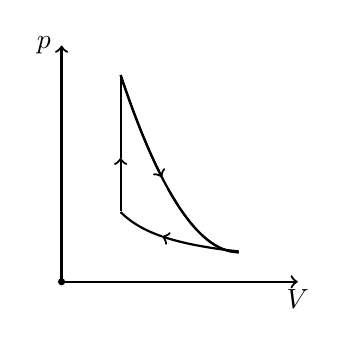
\begin{tikzpicture}
\pgftransformscale{0.75}
	%\draw (0,0) grid (4,4);
	% x-axis
	\draw [thick,->] (0,0) -- (4,0);
	% y-axis
	\draw [thick,->] (0,0) -- (0,4);
	% x-axis label
	\node at (-0.3,4){$p$};
	% y-axis label
	\node at (4,-0.3){$V$};
	% origin point
	\draw [color=black,fill=black] (0,0) circle (0.05);
	%Isokor uppvärmning
	\draw [thick,->](1,1.19) -- (1,2.1);
  \draw [thick](1,2.1) -- (1,3.5);
	%Isentropis expansion
 \draw[ thick,domain=1:3, smooth, variable=\x, black] plot ({\x}, {(0.5+(3.5-0.5)*(abs((\x-3)/(1-3)))^2});
 \draw[ thick,->,domain=1:1.7, smooth, variable=\x, black] plot ({\x}, {(0.5+(3.5-0.5)*(abs((\x-3)/(1-3)))^2});
 \draw[ thick,domain=1.8:3, smooth, variable=\x, black] plot ({\x}, {(0.5+(3.5-0.5)*(abs((\x-3)/(1-3)))^2});
 %Want to use the below instead
 % \coordinate (A) at (1,3.5);
 %\foreach \x in {1,...,3}{
 %   \coordinate (B) at (\x,{(0.5+(3.5-0.5)*(abs((\x-3)/(1-3)))^2});
 %   %\draw[thick, black] (A)--(B) ;
 %   \ifthenelse{\x = 2.5}{\draw[thick,->,smooth, black] (A)--(B) ;}{\draw[thick,smooth, black] (A)--(B) ;}
 %   \coordinate (A) at (B);
 % }
	%Isoterm kompression
	\draw[ thick,->,domain=3:1.7, smooth, variable=\x, black] plot ({\x}, {1/\x + 0.18});
  \draw[ thick,domain=1.7:1, smooth, variable=\x, black] plot ({\x}, {1/\x + 0.18});
   
\end{tikzpicture}
\usetikzlibrary{fit}
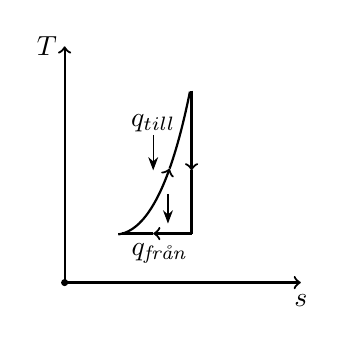
\begin{tikzpicture}[dot/.style={fill=black,circle,minimum size=2pt}]
\pgftransformscale{0.75}
	%\draw (0,0) grid (4,4);
	% x-axis
	\draw [thick,->] (0,0) -- (4,0);
	% y-axis
	\draw [thick,->] (0,0) -- (0,4);
	% x-axis label
	\node at (-0.3,4){$T$};
	% y-axis label
	\node at (4,-0.3){$s$};
	% origin point
	\draw [color=black,fill=black] (0,0) circle (0.05);
	%Isokor uppvärmning
	\draw[ ->,rotate=7,thick,domain=1:2, smooth, variable=\x, black] plot ({\x}, {(0.7 + (\x-1)^2});
  \draw[ rotate=7,thick,domain=2:2.5, smooth, variable=\x, black] plot ({\x}, {(0.7 + (\x-1)^2});
 
 
	%Isentropis expansion
  \draw [thick,->] (2.15,3.25) -- (2.15,1.9);
  \draw [thick] (2.15,1.9) -- (2.15,0.83);
  %Isoterm kompression
  \draw [thick,->] (2.15,0.83) -- (1.5,0.83);
  \draw [thick] (1.5,0.83) -- (0.98,0.83);

  %Pilar
    \usetikzlibrary {arrows.meta}
    \draw [arrows ={-Stealth[scale=1]}] (1.5,2.5) -- (1.5,1.9);
    \draw [arrows ={-Stealth[scale=1]}] (1.75,1.5) -- (1.75,1.0);

     \path (1.5,2.7) node  {$q_{till}$};
     \path (1.6,0.5) node  {$q_{\textit{från}}$};

 
	
   
\end{tikzpicture}

%\end{multicols}

%\listoffigures
%\listoftables
%\tableofcontents

\end{document}